\begin{minipage}{0.68\textwidth}




\only<1>{

Сила в МОЛ:
	\begin{equation*}
		\vc{F} = \frac{\hbar \vc{k} \Gamma}{2}\left(
			\frac{s}{1+s+4\left(\frac{2\pi \delta - \vc{k} \vc{v}}{\Gamma}\right)^2}-
			\frac{s}{1+s+4\left(\frac{2\pi \delta + \vc{k} \vc{v}}{\Gamma}\right)^2}
		\right)
	\end{equation*}

	\begin{figure}[h]
    \centering
    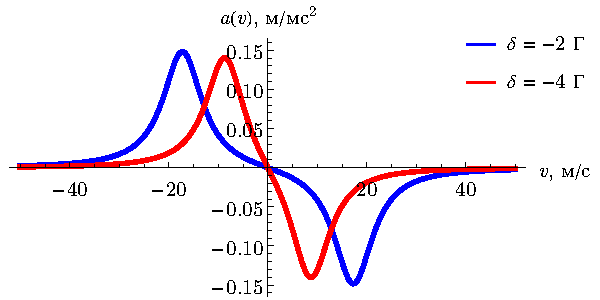
\includegraphics[width=0.8\textwidth]{../MOT/figs/motF.pdf}
    \caption{Зависимость ускорения от силы светового давления, действующей на движущийся атом от его скорости}
    %\label{fig:}
\end{figure}
}

\only<2>{

Сила в МОЛ:
	\begin{equation*}
		\vc{F} = \frac{\hbar \vc{k} \Gamma}{2}\left(
			\frac{s}{1+s+4\left(\frac{2\pi \delta - \vc{k} \vc{v}}{\Gamma}\right)^2}-
			\frac{s}{1+s+4\left(\frac{2\pi \delta + \vc{k} \vc{v}}{\Gamma}\right)^2}
		\right)
	\end{equation*}

	Магнитное поле $\Rightarrow$ эффект Зеемана:
	\begin{equation*}
		\vc{B} = \beta (-x,\,  -y,\, 2z)\T/2,
		\hspace{10 mm} 
		\Delta E = - \vc{B} \vc{\mu},
		\hspace{5 mm} 
		\delta \to \delta + \Delta E /\hbar
	\end{equation*}

	\phantom{42}



	Движение в МОЛ $\sim$ затухающий осциллятор:
	\begin{equation*}
		\vc{F}(\vc{r}, \vc{v}) = -\alpha \vc{v} - \varkappa \vc{r}
	\end{equation*}

	с коэффициентами
	\begin{equation*}
			\varkappa = \frac{-\delta}{\Gamma/2\pi}\frac{8 \subt{\mu}{B} \beta k s}{\left(1+s+4\left(\frac{2\pi \delta}{\Gamma}\right)^2\right)^2},
			\hspace{5 mm} 
			\alpha = \frac{-\delta}{\Gamma} \frac{8 \hbar k^2 s}{\left(1+s+4\left(\frac{2\pi \delta}{\Gamma}\right)^2\right)^2},
	\end{equation*}

}



\end{minipage}
\hfill
\begin{minipage}{0.31\textwidth}

\begin{figure}[h]
    \centering
    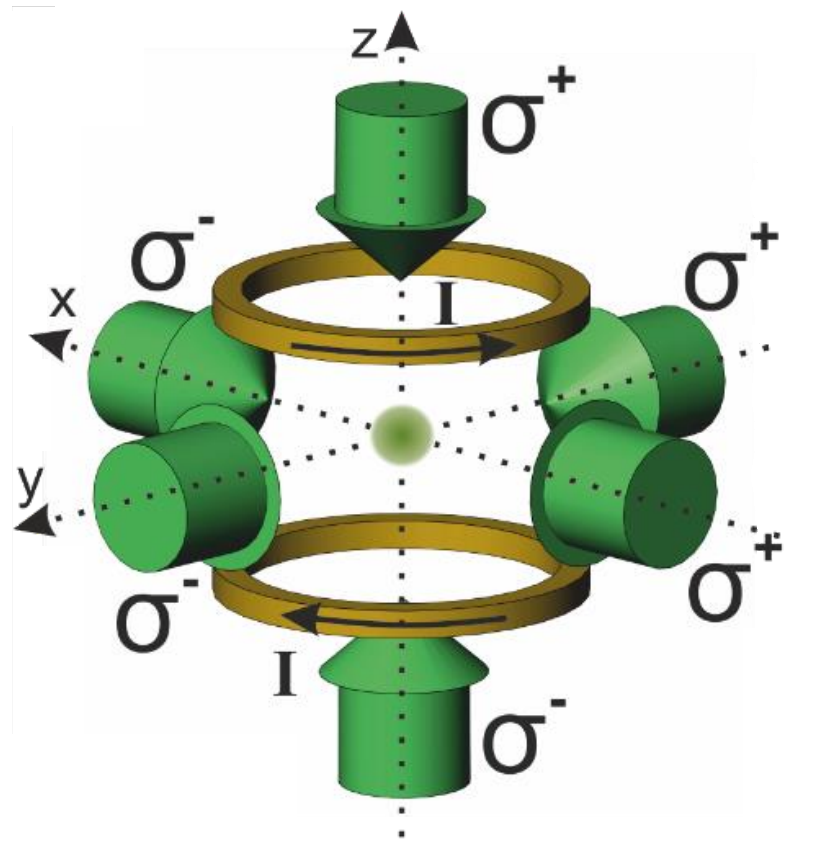
\includegraphics[width=1.0\textwidth]{../MOT/figs/mot.png}
    \caption{Схема лучей МОЛ}
    %\label{fig:}
\end{figure}

\end{minipage}



